\documentclass{article}
\usepackage{geometry}
\usepackage{paralist}
\usepackage[T1]{fontenc}
\usepackage{reledmac}
\usepackage{changepage}

\usepackage{pgfplots}
\usepackage{tikz}
\usetikzlibrary{positioning}
\usetikzlibrary{shapes.geometric, arrows}
\tikzstyle{arrow} = [thick,->,>=stealth]

\usepackage{graphicx}
\graphicspath{ {./images/} }

\usepackage{fancyhdr}
\fancyhead[L]{
	\begin{tabular}{l}
		\Large \textbf{\textsc{Advanced Networking and Future Internet}} \\
		\large Practical Exercise 02
	\end{tabular}
}
\fancyhead[R]{
	\begin{tabular}{r}
		16-124-836 \\
		Marcel \textsc{Zauder}
	\end{tabular}
}
\renewcommand{\headrulewidth}{0.4pt}
\fancyfoot[C]{\thepage}
\renewcommand{\footrulewidth}{0.4pt}

\usepackage{hyperref}

\begin{document}
	\pagestyle{fancy}
	%\hfill
	
	\section*{1.4.1 How many nodes are reachable before and after starting the controller?}
	\begin{adjustwidth}{2em}{2em}
		\subsection*{1.4.1.a Before starting the controller}
		\begin{adjustwidth}{2em}{2em}
		\begin{enumerate}
			\item \textsc{linear} \\
			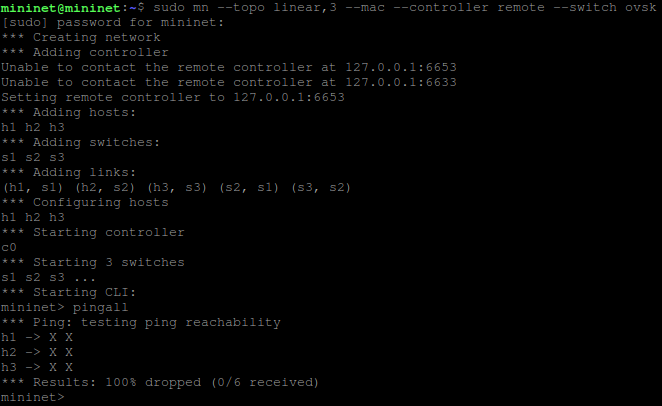
\includegraphics[scale=0.5]{linear_before.png}
			\item \textsc{single} \\
			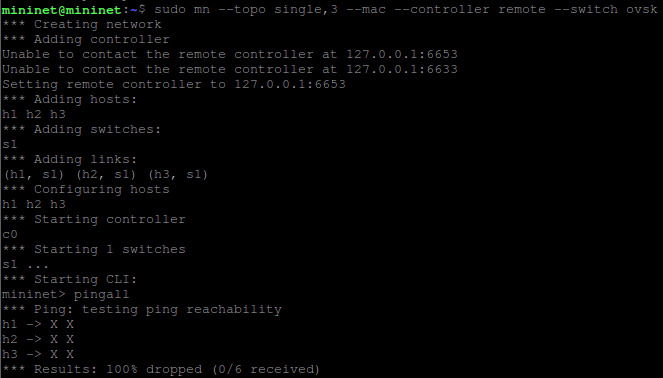
\includegraphics[scale=0.45]{single_before.png}
			\item \textsc{tree} \\
			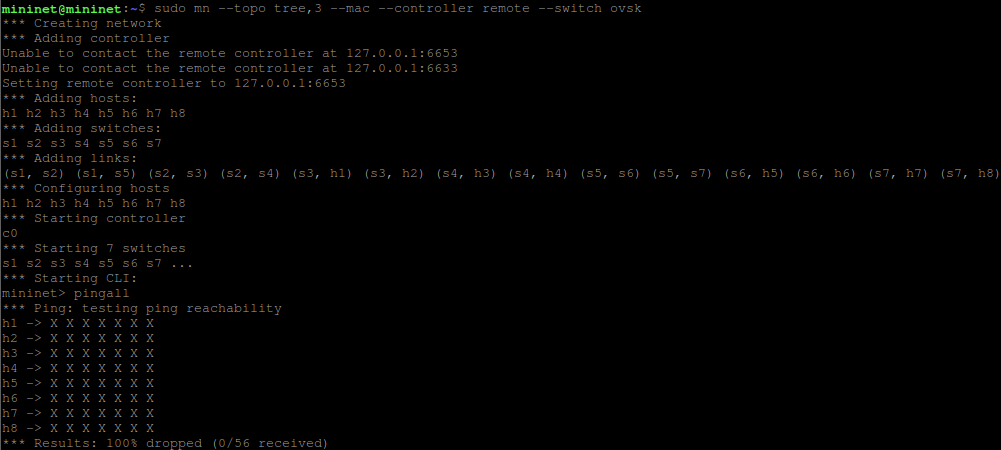
\includegraphics[scale=0.5]{tree_before.png}
		\end{enumerate}
		\end{adjustwidth}
		\subsection*{1.4.1.b After starting the controller}
		\begin{adjustwidth}{2em}{2em} 
		\begin{enumerate}
			\item \textsc{linear} \\
			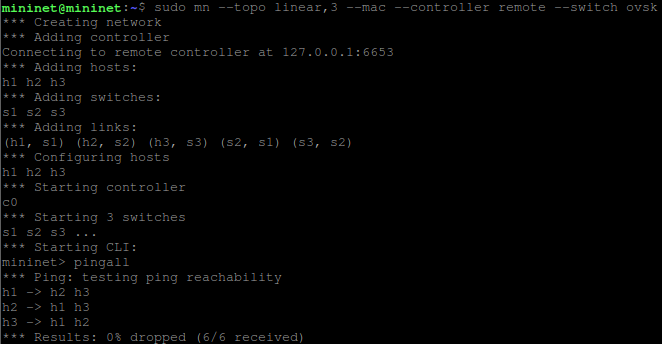
\includegraphics[scale=0.5]{linear_after.png}
			\item \textsc{single} \\
			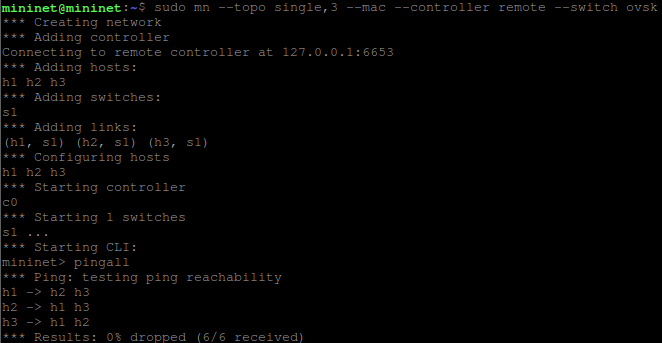
\includegraphics[scale=0.5]{single_after.png}
			\item \textsc{tree} \\
			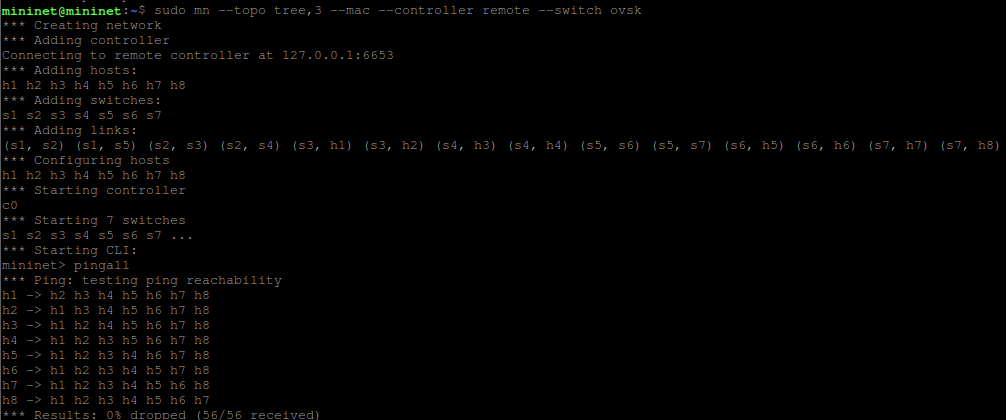
\includegraphics[scale=0.5]{tree_after.png} \\
		\end{enumerate}
		\end{adjustwidth}
		Before setting up the switches none of the hosts can communicate with each other because the packets are dropped instantly at the switches because it is the default behavior. After starting the controller each host can reach the others and communicate with them.
	\end{adjustwidth}
	
	\section*{1.4.2 Flowtables?}
	\begin{adjustwidth}{2em}{2em}
		\begin{enumerate}
			\item \textsc{linear} \\
			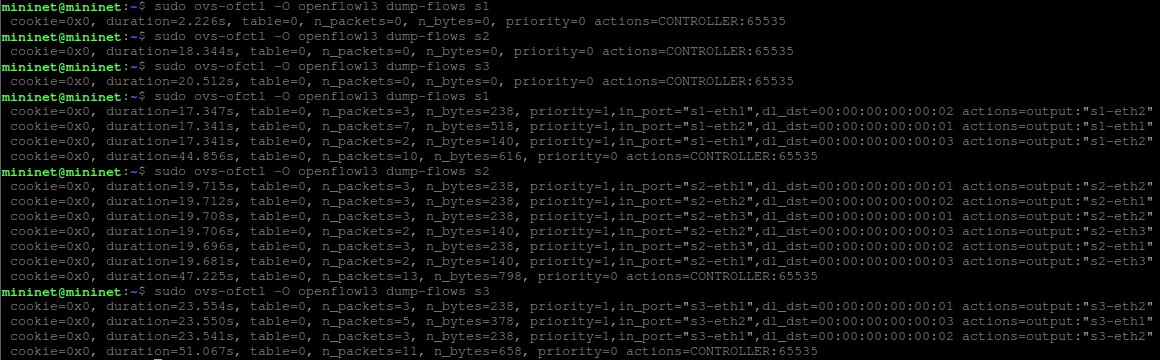
\includegraphics[scale=0.42]{linear_flowtables.png}
			\item \textsc{single} \\
			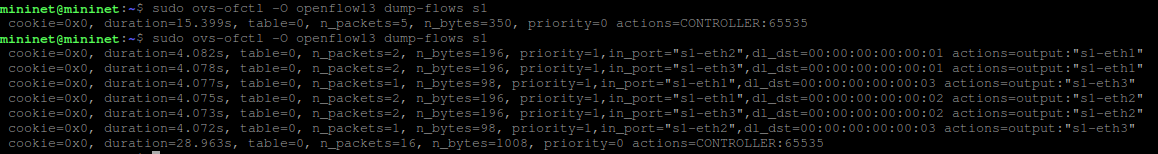
\includegraphics[scale=0.42]{single_flowtables.png}
			\item \textsc{tree} \\
			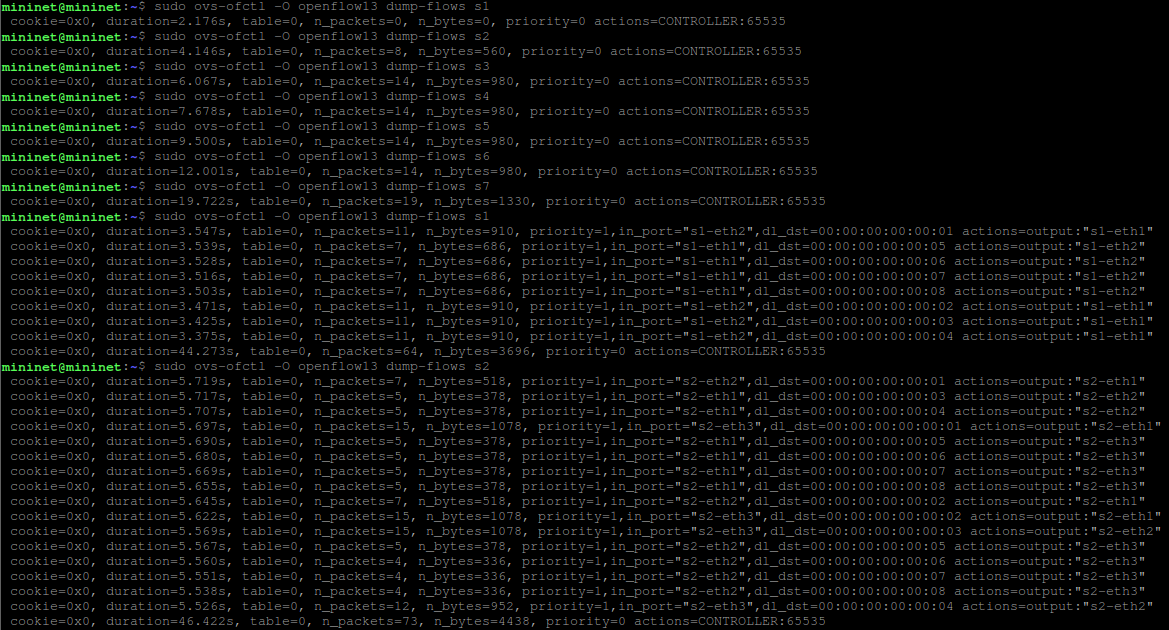
\includegraphics[scale=0.42]{tree_flowtables_1.png} \\
			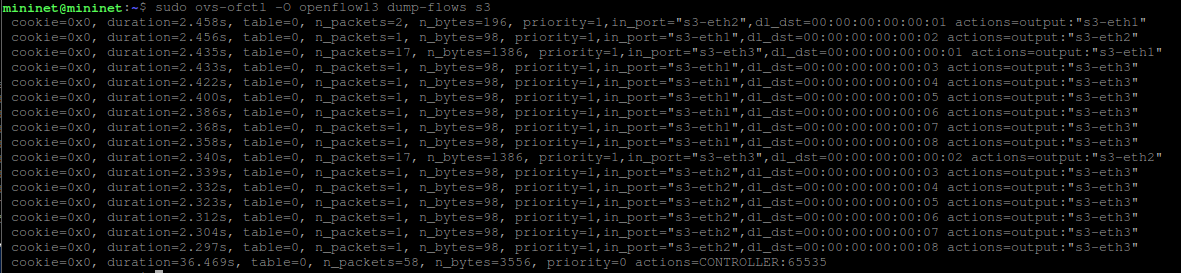
\includegraphics[scale=0.42]{tree_flowtables_2.png} \\
			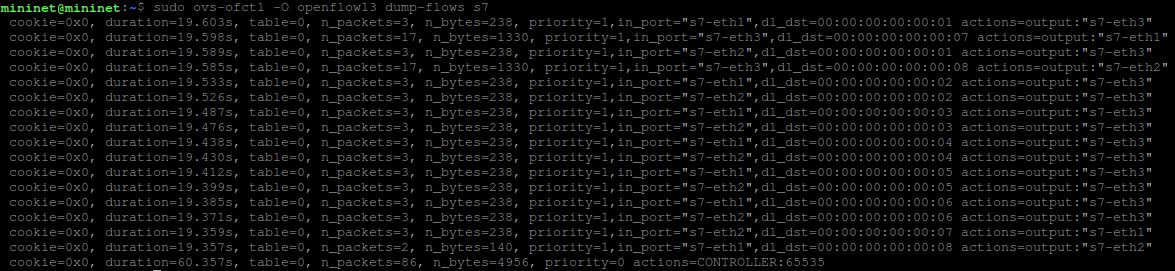
\includegraphics[scale=0.42]{tree_flowtables_3.png} \\
			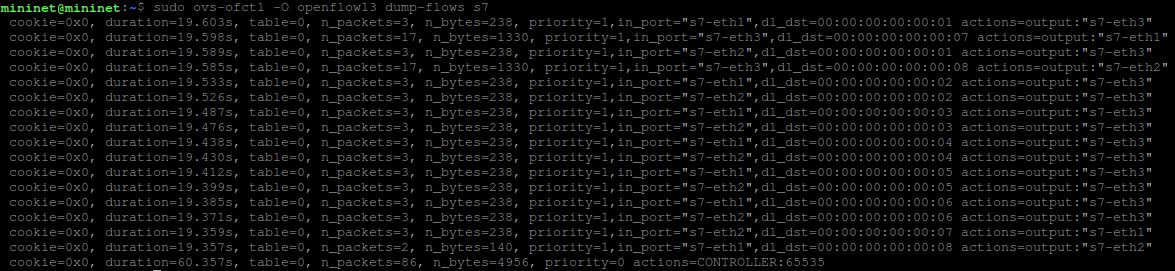
\includegraphics[scale=0.42]{tree_flowtables_4.png}
		\end{enumerate}
		\hfill \\
		In the flowtables we can see that each packet has an in\_port which tells the switch from which port the packet came from. Each of the packets also has the information on where its destination is such that the output port can be computed. So when a packet from one port with a certain destination arrives the switch can lookup in the flowtable to determine which output-port the packet is sent out from. \\
		For example we will follow a packet sent from $h2$ to $h6$ in the tree topology. First the packet arrives at switch $s3$ at the in\_port $s3-eth2$. Because the destination is $00:00:00:00:00:06$ the packet is sent out from port $s3-eth3$. Then the packet arrives at switch $s2$ on in\_port $s2-eth1$ and is sent further from port $s2-eth3$. After arriving at switch $s1$ at in\_port $s1-eth1$ and sent then from $s1-eth2$ to in\_port $s5-eth3$ it is sent to switch $s6$ by using port $s5-eth1$. At $s6$ the packet arrives at in\_port $s6-eth3$ which in the end leads to the packet be sent from port $s6-eth2$ to the node $h6$; arriving at its destination.
	\end{adjustwidth}	
\end{document}